\documentclass[tikz,border=10pt]{standalone}
\usetikzlibrary{arrows.meta, positioning, calc, angles, quotes}
\usepackage{amssymb}

\begin{document}
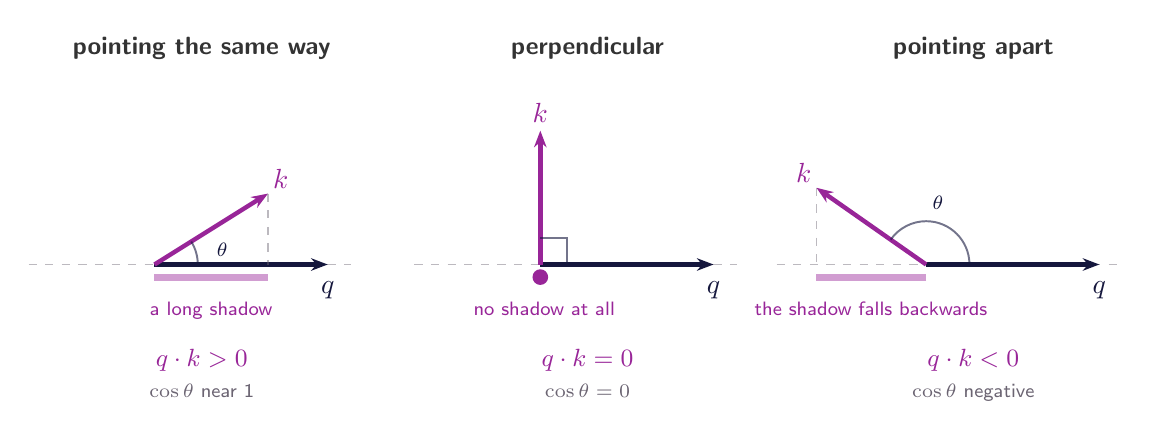
\begin{tikzpicture}[
    every node/.style={font=\sffamily},
]

% ---------------------------------------------------------------- colours
\definecolor{c1}{HTML}{15173D}   % the query
\definecolor{c2}{HTML}{982598}   % the key, and its shadow on the query
\definecolor{c3}{HTML}{E491C9}
\definecolor{c4}{HTML}{F1E9E9}
\definecolor{axiscolor}{HTML}{333333}
\definecolor{labelcolor}{HTML}{6B6472}

\tikzset{
    qvec/.style={-{Stealth[length=6pt]}, line width=1.6pt, c1},
    kvec/.style={-{Stealth[length=6pt]}, line width=1.6pt, c2},
    shadow/.style={line width=2.6pt, c2, opacity=0.45},
    guide/.style={labelcolor, opacity=0.45, dashed, line width=0.6pt},
}

% ================================================================
% Three panels, same q, k turned further round each time.
%   |q| = 2.2 along +x,  |k| = 1.7
%   panel shifts: 0, 4.9, 9.8
% ================================================================

% ----------------------------------------------------------------------
% PANEL 1: theta small
%   k at 32 deg  ->  tip (1.442, 0.901), foot at x = 1.442
% ----------------------------------------------------------------------
\begin{scope}[shift={(0, 0)}]
    \node[font=\sffamily\small\bfseries, text=axiscolor] at (0.6, 2.75)
        {pointing the same way};

    \draw[guide] (-1.6, 0) -- (2.5, 0);
    \draw[qvec] (0, 0) -- (2.2, 0) node[anchor=north, yshift=-2pt] {$q$};
    \draw[kvec] (0, 0) -- (1.442, 0.901) node[anchor=south west, inner sep=1pt] {$k$};

    \draw[guide] (1.442, 0.901) -- (1.442, 0);
    \draw[shadow] (0, -0.16) -- (1.442, -0.16);

    \draw[c1, opacity=0.6, line width=0.7pt] (0.55, 0) arc (0:32:0.55);
    \node[font=\sffamily\scriptsize, text=c1] at (0.86, 0.19) {$\theta$};

    \node[font=\sffamily\scriptsize, text=c2, anchor=north] at (0.72, -0.35)
        {a long shadow};
    \node[font=\sffamily\small\bfseries, text=c2, anchor=north] at (0.6, -0.95)
        {$q \cdot k > 0$};
    \node[font=\sffamily\scriptsize, text=labelcolor, anchor=north]
        at (0.6, -1.4) {$\cos\theta$ near 1};
\end{scope}

% ----------------------------------------------------------------------
% PANEL 2: right angle
% ----------------------------------------------------------------------
\begin{scope}[shift={(4.9, 0)}]
    \node[font=\sffamily\small\bfseries, text=axiscolor] at (0.6, 2.75)
        {perpendicular};

    \draw[guide] (-1.6, 0) -- (2.5, 0);
    \draw[qvec] (0, 0) -- (2.2, 0) node[anchor=north, yshift=-2pt] {$q$};
    \draw[kvec] (0, 0) -- (0, 1.7) node[anchor=south, inner sep=2pt] {$k$};

    \draw[c1, opacity=0.6, line width=0.7pt]
        (0.34, 0) -- (0.34, 0.34) -- (0, 0.34);

    \node[circle, fill=c2, inner sep=2pt] at (0, -0.16) {};
    \node[font=\sffamily\scriptsize, text=c2, anchor=north] at (0.05, -0.35)
        {no shadow at all};
    \node[font=\sffamily\small\bfseries, text=c2, anchor=north] at (0.6, -0.95)
        {$q \cdot k = 0$};
    \node[font=\sffamily\scriptsize, text=labelcolor, anchor=north]
        at (0.6, -1.4) {$\cos\theta = 0$};
\end{scope}

% ----------------------------------------------------------------------
% PANEL 3: obtuse
%   k at 145 deg  ->  tip (-1.393, 0.975), foot at x = -1.393
% ----------------------------------------------------------------------
\begin{scope}[shift={(9.8, 0)}]
    \node[font=\sffamily\small\bfseries, text=axiscolor] at (0.6, 2.75)
        {pointing apart};

    \draw[guide] (-1.9, 0) -- (2.5, 0);
    \draw[qvec] (0, 0) -- (2.2, 0) node[anchor=north, yshift=-2pt] {$q$};
    \draw[kvec] (0, 0) -- (-1.393, 0.975) node[anchor=south east, inner sep=1pt] {$k$};

    \draw[guide] (-1.393, 0.975) -- (-1.393, 0);
    \draw[shadow] (0, -0.16) -- (-1.393, -0.16);

    \draw[c1, opacity=0.6, line width=0.7pt] (0.55, 0) arc (0:145:0.55);
    \node[font=\sffamily\scriptsize, text=c1] at (0.15, 0.78) {$\theta$};

    \node[font=\sffamily\scriptsize, text=c2, anchor=north] at (-0.7, -0.35)
        {the shadow falls backwards};
    \node[font=\sffamily\small\bfseries, text=c2, anchor=north] at (0.6, -0.95)
        {$q \cdot k < 0$};
    \node[font=\sffamily\scriptsize, text=labelcolor, anchor=north]
        at (0.6, -1.4) {$\cos\theta$ negative};
\end{scope}

% the takeaway lives in the figcaption, not inside the figure

\end{tikzpicture}
\end{document}
